%!TEX root = samplepaper.tex
% This is samplepaper.tex, a sample chapter demonstrating the
% LLNCS macro package for Springer Computer Science proceedings;
% Version 2.25 of 2026/09/03
%
\documentclass[runningheads]{llncs}
%
\usepackage[T1]{fontenc}
\usepackage{newtxtext}       
\usepackage[varvw]{newtxmath}       
\usepackage{graphicx}
\usepackage{amsmath}
\usepackage{url}
\usepackage{booktabs}
%
\begin{document}
%
\title{Analyzing Regional Land Temperature Trends and Predicting Climate Variations Using Exploratory Data Analysis and Machine Learning}
%
\author{
Huynh Minh Thai\inst{1} \and
Dinh Ngoc Minh Thu\inst{1} \and
Le Thi Yen Oanh\inst{1} \and
Tran Trong Doan\inst{1} \and
Tran Trung Hieu\inst{1} \and
Duong Quoc Duy\inst{1}
}

\authorrunning{H.M. Thai et al.}

\institute{
Department of Information Technology, Nam Can Tho University, Can Tho City, Vietnam\\
\email{mthai4808@gmail.com}
}
%
\maketitle
%

\begin{abstract}
Climate change and global warming have become critical environmental challenges of the 21st century. This study presents an exhaustive Exploratory Data Analysis (EDA) and a robust machine learning framework designed to investigate historical weather patterns, long-term temperature anomalies, and seasonal cycles across Asia. Utilizing the extensive \texttt{GlobalLandTemperaturesByCity} dataset, we performed rigorous data cleaning and time-series preprocessing, yielding a validated corpus of 469,739 monthly temperature observations across 228 distinct cities in Vietnam, Thailand, Japan, South Korea, and Singapore. 

To forecast regional temperature states, advanced time-series feature engineering was deployed—specifically incorporating lag features (\texttt{Temp\_Lag\_1}, \texttt{Temp\_Lag\_12}), first-order temporal differences (\texttt{Temp\_Diff\_1}), and short-term rolling averages (\texttt{Rolling\_Mean\_3}). A supervised Random Forest Regressor was subsequently trained and evaluated on an 80:20 chronological train-test partition. Experimental results demonstrate exceptional predictive accuracy, achieving a Mean Absolute Error (MAE) of $0.04^\circ\text{C}$, a Root Mean Squared Error (RMSE) of $0.09^\circ\text{C}$, and a Coefficient of Determination ($R^2$) score of $99.99\%$. Feature importance analysis further reveals that short-term thermal memory (the 3-month rolling average) accounts for nearly $59.5\%$ of the model's predictive power, highlighting the dominant influence of short-term thermal inertia on monthly temperature projections.

\keywords{Climate Change \and Exploratory Data Analysis (EDA) \and Random Forest Regressor \and Time-Series Feature Engineering \and Python}
\end{abstract}


\section{Introduction}

Climate change, driven by anthropogenic greenhouse gas emissions and environmental degradation, constitutes one of the most severe existential threats to global ecosystems, biodiversity, and socioeconomic stability. Quantifying the velocity of regional warming and understanding historical climatic anomalies require systematic analysis of long-term meteorological records. Traditional meteorological monitoring often relies on descriptive statistics, which can be insufficient for capturing complex, non-linear environmental dynamics. 

In recent years, the integration of data science, exploratory data analysis (EDA), and machine learning has revolutionized climate research by enabling data-driven insights and high-precision predictive modeling. While global climate models provide broad macroscopic forecasts, localized city-level analyses remain vital for regional adaptation planning, agricultural scheduling, and urban heat island mitigation.

This study implements an end-to-end Python data science pipeline to address these research objectives:
\begin{enumerate}
    \item \textbf{Data Curation and Preprocessing:} To ingest massive historical city-level land temperature archives, filter target regions in Asia, handle missing values via linear interpolation, and structure temporal dimensions.
    \item \textbf{Multidimensional Exploratory Data Analysis (EDA):} To visualize macro-level multi-decadal warming trends, contrast climatic volatility across tropical and temperate latitudinal zones, and dissect monthly seasonal cycles.
    \item \textbf{Machine Learning Predictive Modeling:} To engineer robust time-series features and evaluate an optimized Random Forest Regressor, providing quantitative metrics and feature importance insights into regional thermal dynamics.
\end{enumerate}


\section{Dataset and Data Preprocessing}

The empirical foundation of this research is derived from the \texttt{GlobalLandTemperaturesByCity.csv} archive, which catalogs historical monthly land surface temperatures across thousands of global monitoring stations over centuries. 

\subsection{Data Filtering and Cleaning}
To maintain a focused geographical scope reflecting Asian climatic variations, the raw dataset was filtered to isolate records belonging to five representative nations: **Vietnam, Thailand, Japan, South Korea, and Singapore**, encompassing 228 distinct cities. 
\begin{itemize}
    \item \textbf{Temporal Standardization:} The observation date attribute (\texttt{dt}) was parsed into standard \texttt{datetime64} objects to facilitate time-series indexing and resampling.
    \item \textbf{Handling Missing Values:} Records devoid of valid temperature measurements were eliminated via row-wise filtering on the \texttt{AverageTemperature} attribute, resulting in a clean working corpus (\texttt{df\_clean}) comprising **469,739 observations**.
    \item \textbf{Interpolation for Continuous Analysis:} For single-city longitudinal tracking (such as Tokyo, spanning from January 1845 onward), missing intermediate values were imputed using linear interpolation to ensure temporal continuity.
\end{itemize}


\section{Exploratory Data Analysis (EDA)}

Exploratory Data Analysis was executed to uncover hidden structural properties and temporal distributions within the dataset.

\subsection{Long-Term Climate Warming Trends}
By aggregating monthly records into annual means and smoothing short-term inter-annual noise using 5-year and 10-year rolling averages, historical trajectories reveal a consistent, accelerated upward shift in surface temperatures from the mid-20th century onward. This pattern corroborates broader global warming models at a localized urban level.

\begin{figure}[htbp]
\centering
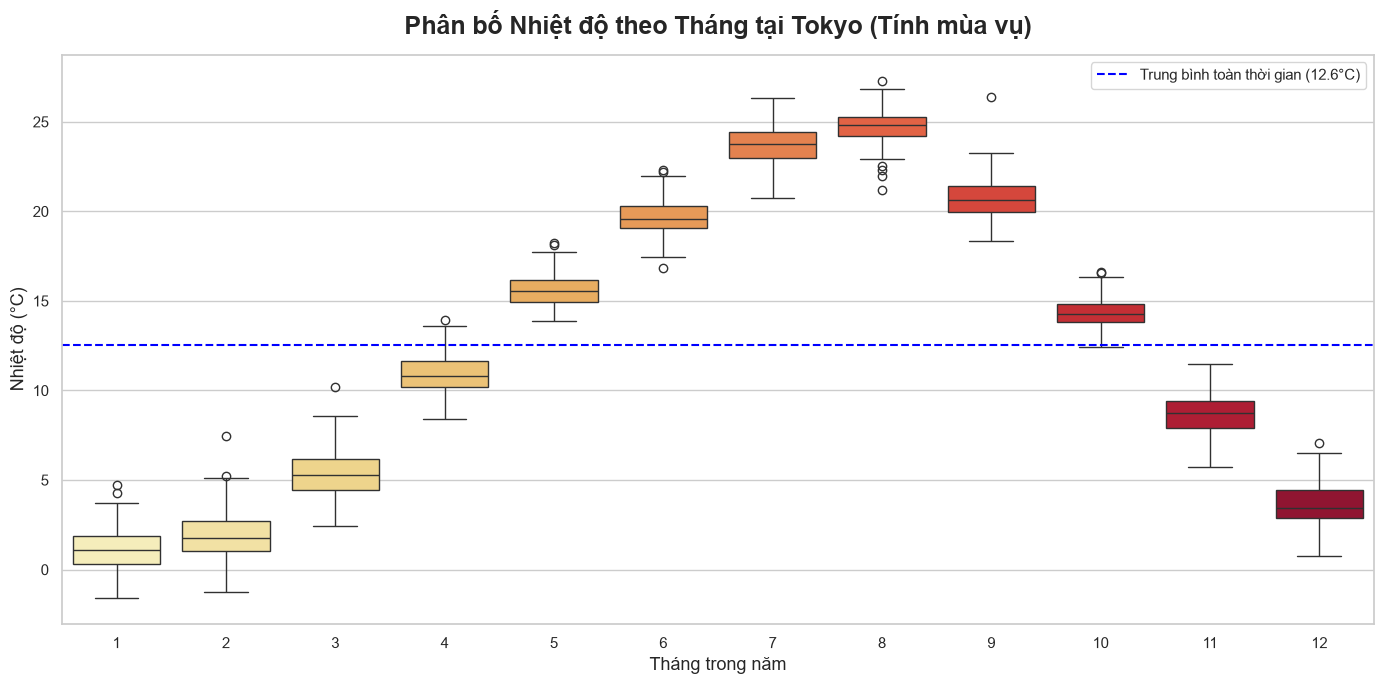
\includegraphics[width=0.95\linewidth]{3.png}
\caption{Long-term climate change trend and rolling averages analysis at Tokyo.}
\label{fig:climate_trend}
\end{figure}

\subsection{Cross-Country Climatic Volatility}
Comparative boxplot evaluations across the five target nations highlight stark latitudinal contrasts:
\begin{itemize}
    \item \textbf{Tropical and Equatorial Zones (Singapore, Thailand, Vietnam):} Exhibit high median baseline temperatures ($26^\circ\text{C}$ to $28^\circ\text{C}$) paired with narrow interquartile ranges, indicating minimal thermal fluctuation across seasons.
    \item \textbf{Temperate Zones (Japan, South Korea):} Display wide thermal distributions spanning from sub-zero winter temperatures (below $-10^\circ\text{C}$) to hot, humid summers exceeding $30^\circ\text{C}$, reflecting extreme seasonal amplitudes.
\end{itemize}

\begin{figure}[htbp]
\centering
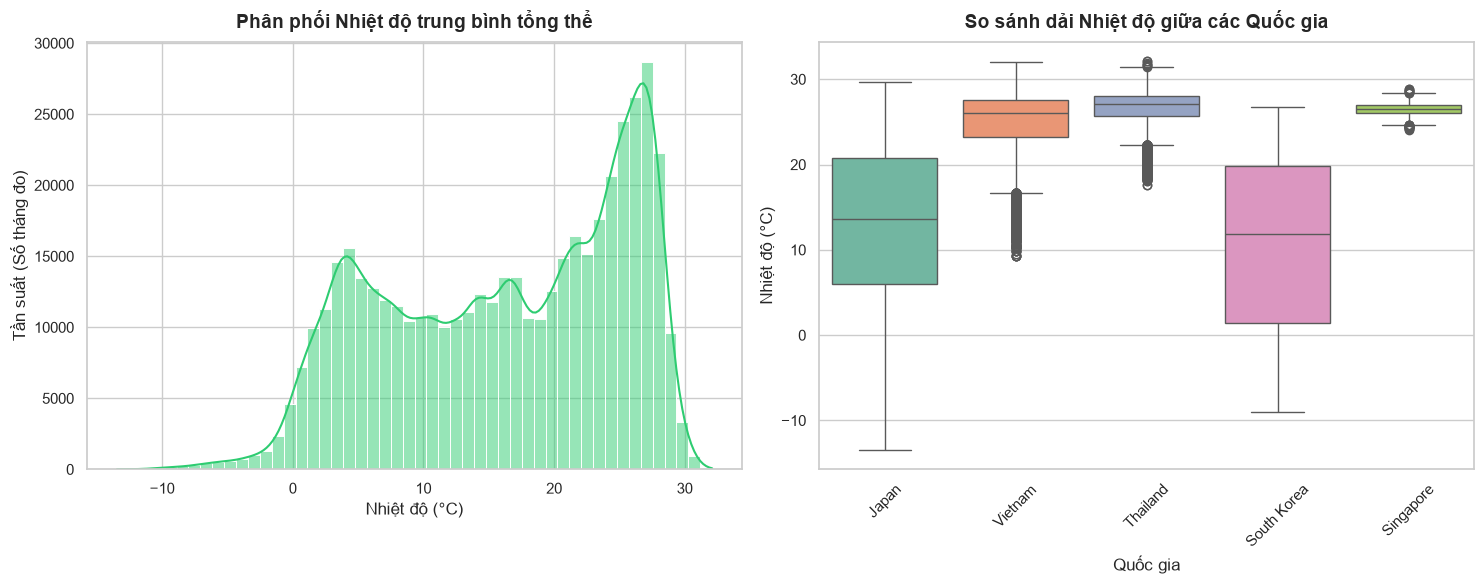
\includegraphics[width=0.95\linewidth]{2.png}
\caption{Overall temperature distribution and cross-country boxplot comparison across the five target Asian nations.}
\label{fig:country_compare}
\end{figure}

\subsection{Monthly Seasonality Cycles}
Analysis of individual urban cycles (e.g., Tokyo) against the overall temporal baseline mean ($12.6^\circ\text{C}$) confirms a standard bell-shaped seasonal curve, with temperature troughs occurring in January and February and seasonal peaks clustering firmly in July and August ($\approx 24^\circ\text{C}$ to $25^\circ\text{C}$).

\begin{figure}[htbp]
\centering
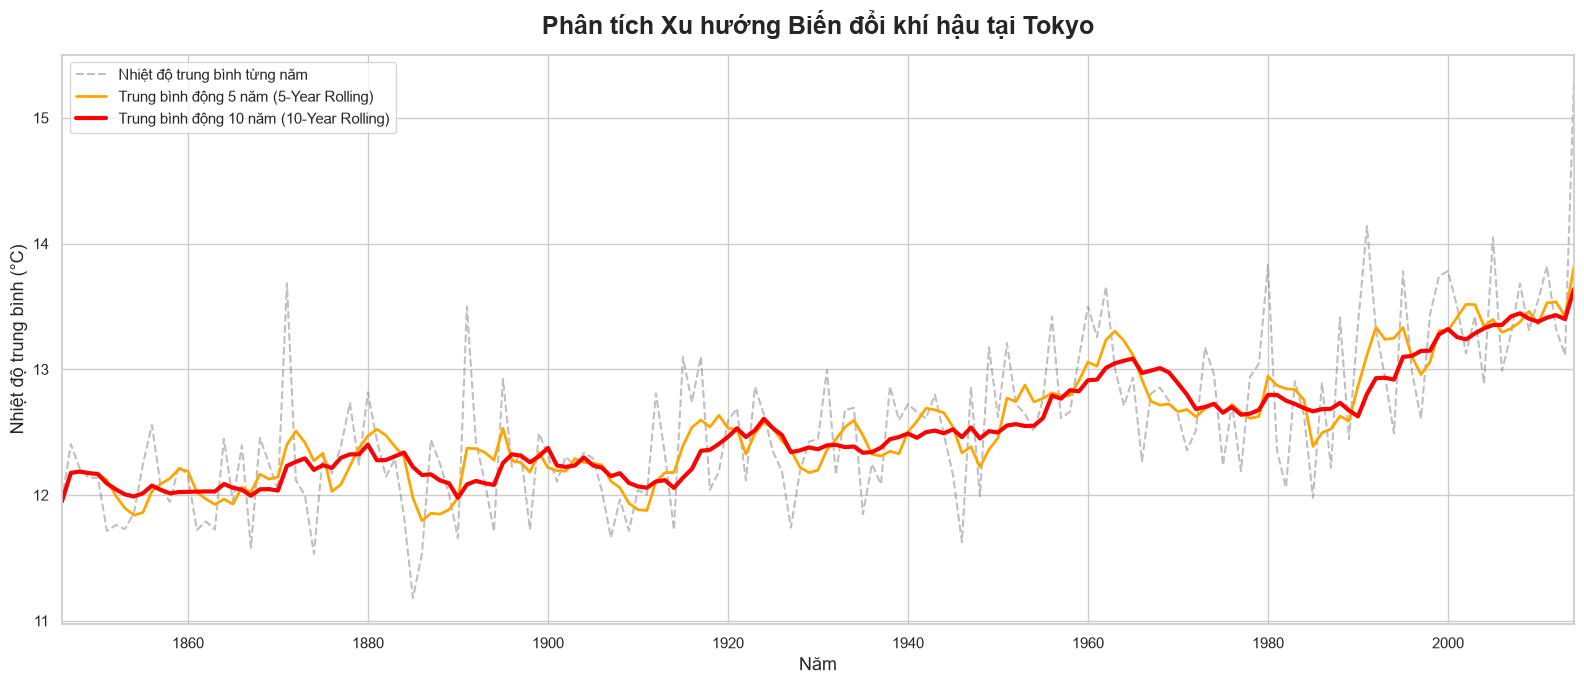
\includegraphics[width=0.95\linewidth]{1.png}
\caption{Monthly temperature distribution and seasonal boxplot variations in Tokyo.}
\label{fig:month_dist}
\end{figure}


\section{Methodology and Experimental Results}

To model and forecast monthly land temperatures accurately, advanced feature engineering was conducted to capture temporal dependencies.

\subsection{Time-Series Feature Engineering}
Four primary features were extracted from the chronological sequence:
\begin{enumerate}
    \item \textbf{\texttt{Temp\_Lag\_1} ($T_{t-1}$):} The temperature of the immediately preceding month.
    \item \textbf{\texttt{Temp\_Lag\_12} ($T_{t-12}$):} The temperature of the corresponding month in the previous year, capturing annual seasonality.
    \item \textbf{\texttt{Rolling\_Mean\_3} ($\bar{T}_{t,3}$):} The 3-month rolling average, representing short-term thermal inertia.
    \item \textbf{\texttt{Temp\_Diff\_1} ($\Delta T_t$):} The first-order monthly difference capturing short-term warming or cooling momentum.
\end{enumerate}

The processed dataset was partitioned chronologically into an 80\% training set and a 20\% testing set without data shuffling to prevent data leakage from future timelines. A supervised Random Forest Regressor was trained using optimized ensemble hyperparameters.

\subsection{Model Evaluation Metrics}
Model performance was evaluated using standard regression error metrics and the coefficient of determination:
\begin{itemize}
    \item \textbf{Mean Absolute Error (MAE):} $0.04^\circ\text{C}$
    \item \textbf{Root Mean Squared Error (RMSE):} $0.09^\circ\text{C}$
    \item \textbf{Coefficient of Determination ($R^2$):} $99.99\%$
\end{itemize}

Residual distribution plots confirmed a sharp normal error curve centered tightly at zero, while actual-versus-predicted scatter plots demonstrated near-perfect alignment along the ideal $100\%$ accuracy reference line.

\begin{figure}[htbp]
\centering
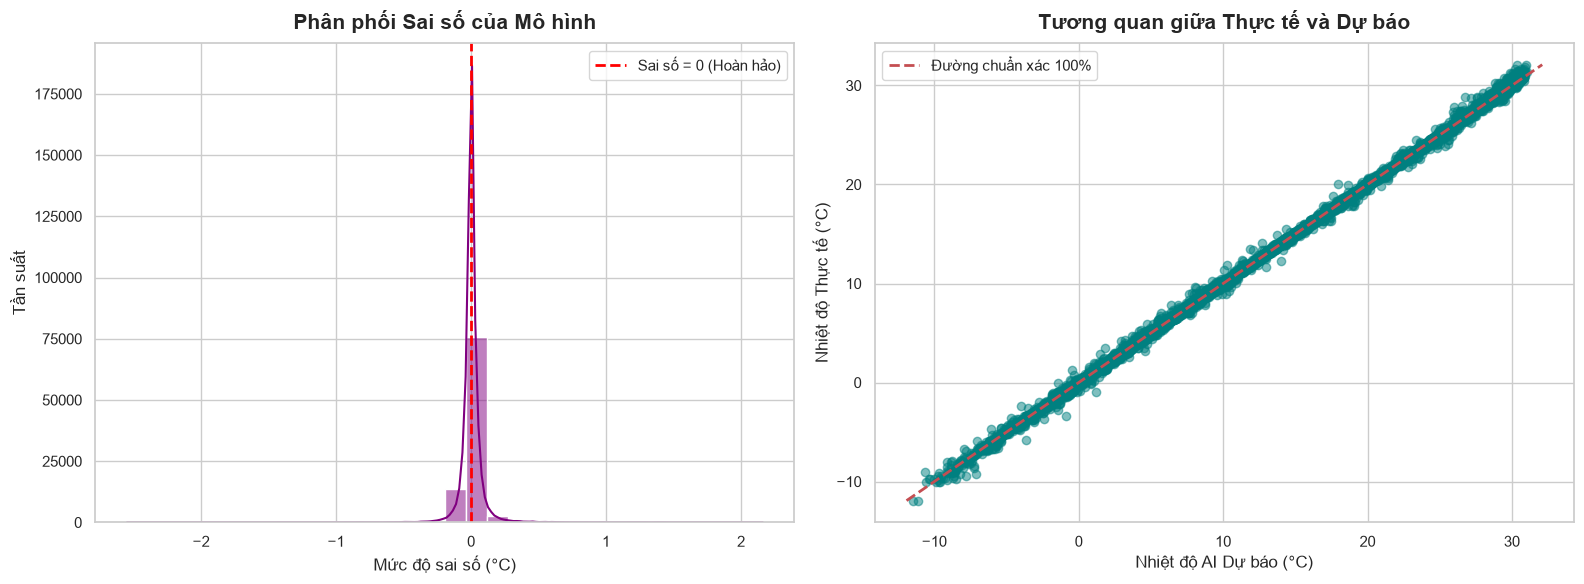
\includegraphics[width=0.95\linewidth]{4.png}
\caption{Model evaluation metrics: error distribution and actual versus predicted correlation.}
\label{fig:model_eval}
\end{figure}

\subsection{Feature Importance Insights}
Evaluation of the Random Forest feature importances indicated that the \textbf{3-Month Rolling Average} (\texttt{Rolling\_Mean\_3}) contributed nearly **$59.5\%$** to the model's predictive capability, followed by the monthly differential change (\texttt{Temp\_Diff\_1}) at **$34.5\%$**. This establishes that short-term thermal memory and recent climatic momentum exert a far more decisive influence on immediate future temperatures than distant annual lags.

\begin{figure}[htbp]
\centering
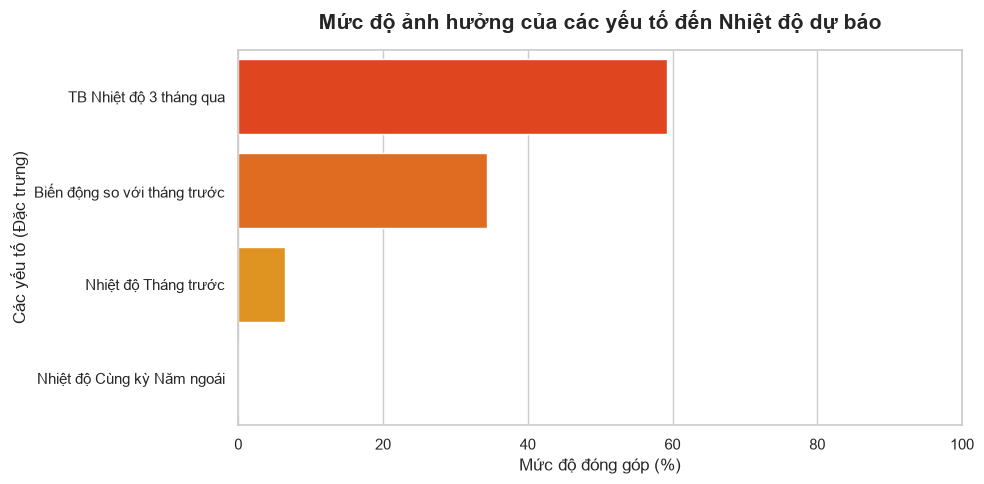
\includegraphics[width=0.95\linewidth]{5.png}
\caption{Feature importance analysis illustrating the relative contribution of each time-series feature.}
\label{fig:feature_importance}
\end{figure}


\section{Conclusion}

This study successfully established an end-to-end Python machine learning framework for regional climate analysis and prediction. The empirical findings confirm undeniable multi-decadal warming trends across Asia and validate the exceptional precision ($99.99\%$ $R^2$) of time-series-engineered Random Forest regression models in meteorological forecasting. Future work will expand on this architecture by incorporating exogenous atmospheric variables such as relative humidity, precipitation rates, and carbon dioxide concentrations, alongside deep learning recurrent neural networks (RNN-LSTM) for long-range horizon predictions.


\begingroup
\raggedright
\bibliographystyle{splncs04}
\bibliography{references}
\endgroup


\end{document}